\chapter{Integrated Photonics}
\label{ch:Integrated_Photonics}

To build an artificial neuromorphic network one has to choose first some physical phenomenon to employ in the fundamental blocks, likewise transistors in electronic circuits use the various behaviors of electrons in resistances, capacitors, and inductances.
The physics which I want to build my artificial neuromorphic network with is photonics, precisely integrated photonics.

Photonics is the physical science which studies detection, manipulation, and emission of light.
Specificially, integrated photonics is the branch that studies how to reduce and \textit{integrate} once macroscopic optical devices in miniaturized structures.
In the past few decades, driven by the growing needs of communication technology, which was in turn following the increase in computational power of electronics, many integrated devices have been proposed and commercialized.

% Many other devices such as Mach-Zenhder interferometers (MZI) and Directional Couplers (DC) have been demonstrated.
% , Arrayed Waveguide Gratings (AWG) and Multimode interference(MMI)
%\subsection{History}

%\subsection{Comparison with other technologies}
\subsection{Silicon Photonics ?}


\section{Guided-wave photonics}
\label{sec:guided-wave_photonics}
The most important thing for integrated photonics is the way light is confined and manipulated into microscopic structures.
While in conventional optics, light is delivered with bulky mirrors and lenses toward the desired position, in integrated photonics waveguides are the main device for the task.

\subsection{Waveguides}
\label{ssec:waveguides}
A waveguide is a path inside a medium, whose volume is defined by a certain number of interfaces between different materials, in which light remains confined and ideally travels with negligible losses.
This volume is called \textit{core} of the waveguide, while the medium external to it, if present, is called \textit{cladding.}

One can distinguish two main types of waveguides: metallic and dielectric.
The former are based on the reflection of the electromagnetic field by the metallic surface.
However, for visible and infrared frequencies, metallic waveguides are not possible, due to too high absorption of the metals at optical frequencies.
On the other hand, dielectric waveguides are based on the phenomenon of total internal reflection (TIR) on the interface between two dielectric media.
To produce TIR, the two materials must have sufficiently different real part of the refractive index.
Moreover, they must also be transparent in the required range of frequencies.
Hence not all media are suitable to build dielectric waveguides that work at a specific wavelength.
For example, silicon is known to be transparent for light at and around \SI{1.55}{\um}, among other wavelengths.
This feature together with a low distortion of signals is the reason why it is the most used wavelength in communication technology.
%The latter are based on the phenomenon of total internal reflection (TIR), and are nowadays widely used \ref{} in the industry and various research fields.

\subsubsection{Dielectric Waveguides}
\label{sssec:Dielectric_Waveguides}
Total internal reflection is the well-known phenomenon in which light coming from a material with high refractive index $n_H$ gets reflected at the interface with a material with low refractive index $n_L$.
For this to happen, incident light must be at an angle greater than the critical angle\index{critical angle} given by the Snell's law\index{Snell's law}:
\begin{equation*}
	\theta_C = \arcsin \left( \dfrac{n_L}{n_H}\right).
\end{equation*}

Waveguides have many shapes, however one can initially discriminate them by the dimensionality of the confinement of light.
The simplest one is called \textit{slab} and it is composed by two interfaces, which divides the material in three volumes, as shown in \autoref{fig:slabVG} below.
This type is classified as a 1D-waveguide, because it constrains light in only one dimension.

\begin{figure}[ht]
	\centering
%	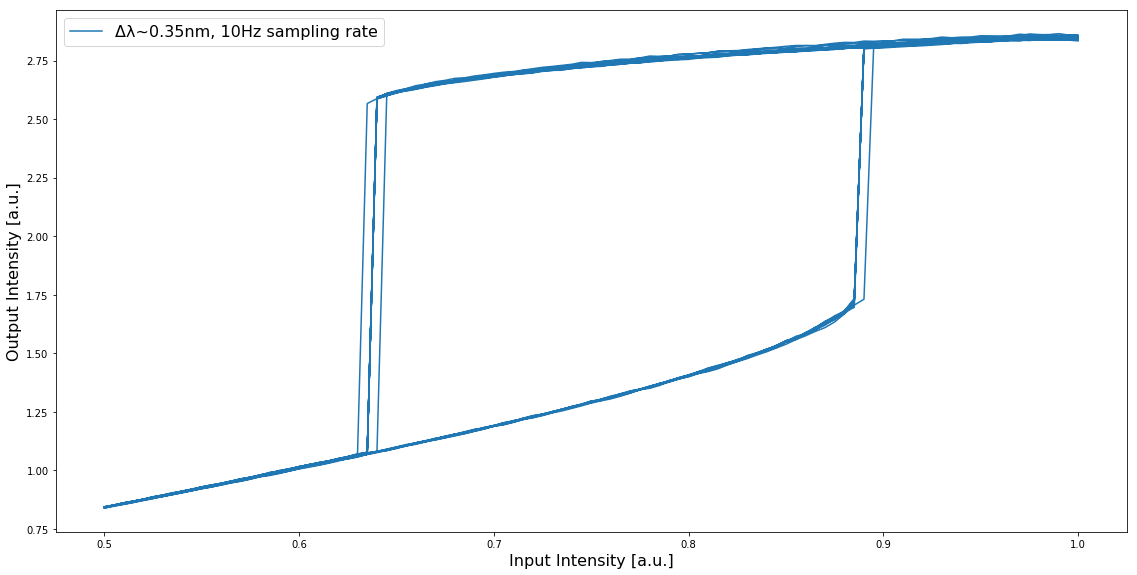
\includegraphics[draft,width=9cm,height=6cm]{figures/foo.png}
	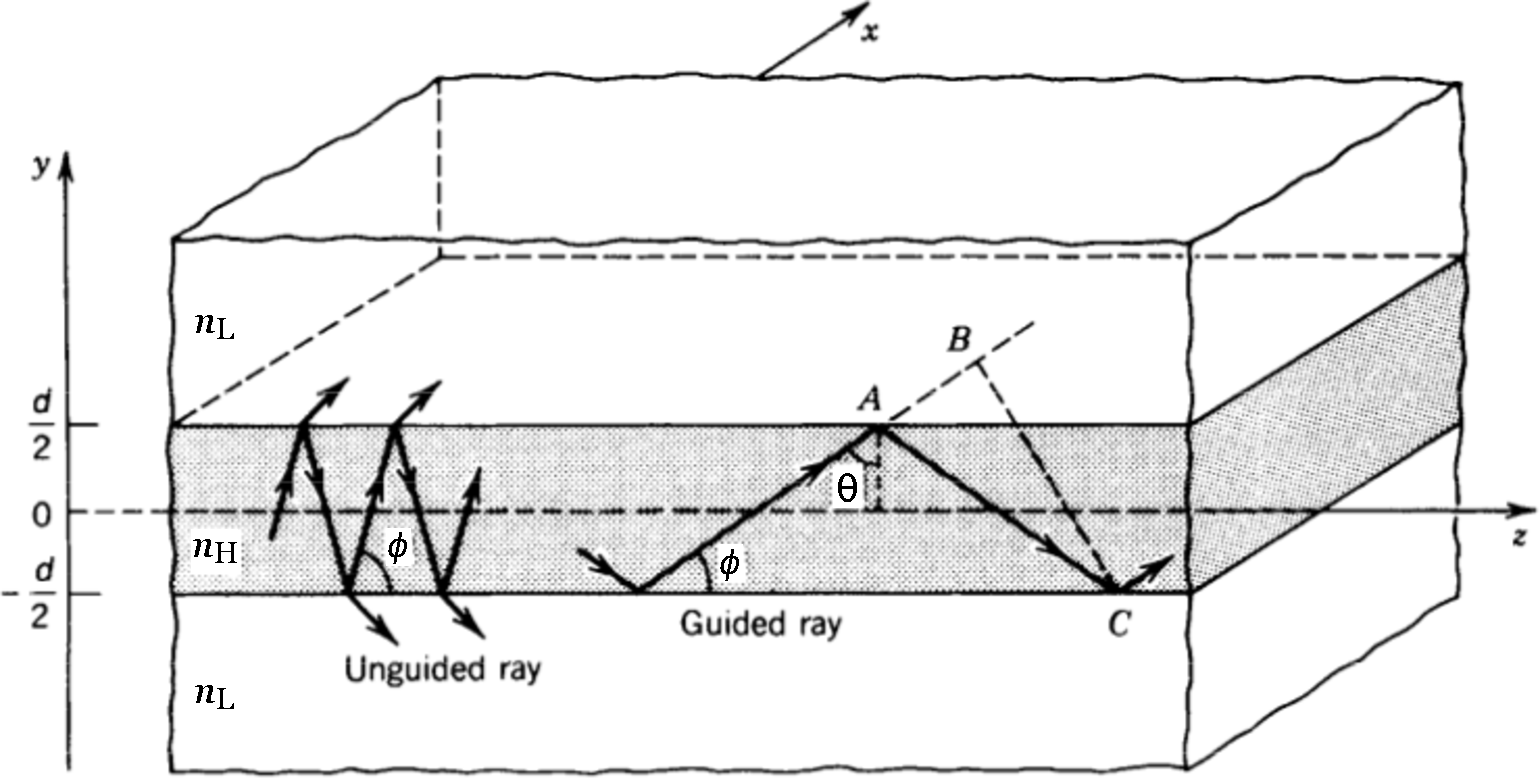
\includegraphics[scale=.4]{figures/dielBC.pdf}
	\caption{Scheme of a dielectric slab waveguide, made by two materials with refractive indexes $n_H$ and $n_L$.
		Two rays are shown: the unguided one is incident on the interface at an angle smaller than the critical angle.
		Conversely the guided ray is incident at an greater angle and is therefore totally reflected inside the waveguide \cite{Saleh1991}.}
	\label{fig:slabVG}
\end{figure}

2D-waveguides on the other hand are more common, to the point that with the term waveguide one usually refers to a device belonging to this category.
Since they confine light in two dimension, their core then becomes a straight path with which one can conduct light from a place to another.
A few types are shown in \autoref{fig:2DVG} below.

\begin{figure}[ht]
	\centering
%	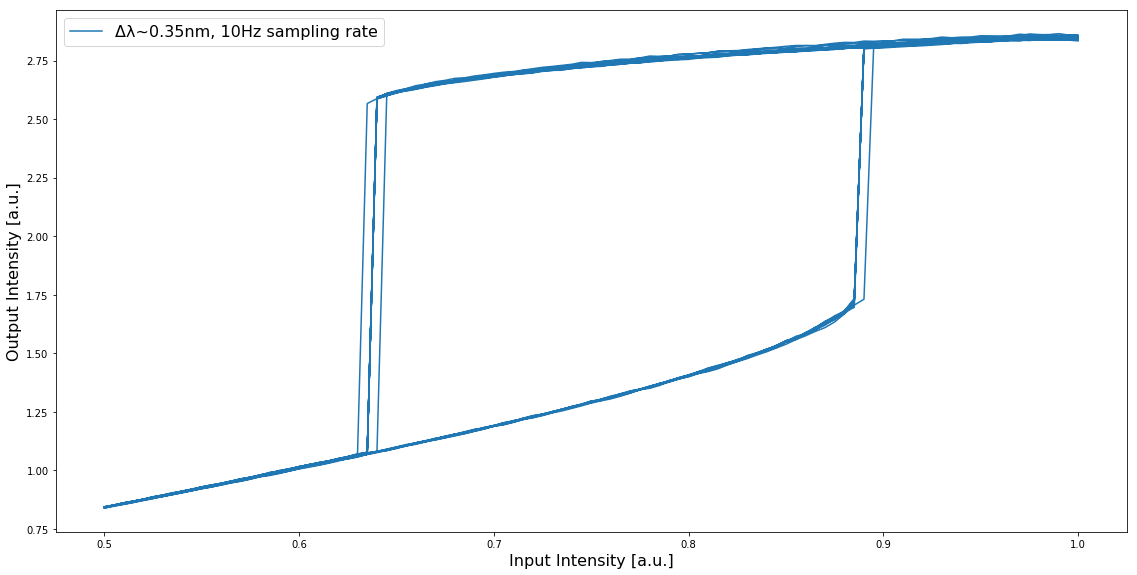
\includegraphics[draft,width=9cm,height=6cm]{figures/foo.png}
	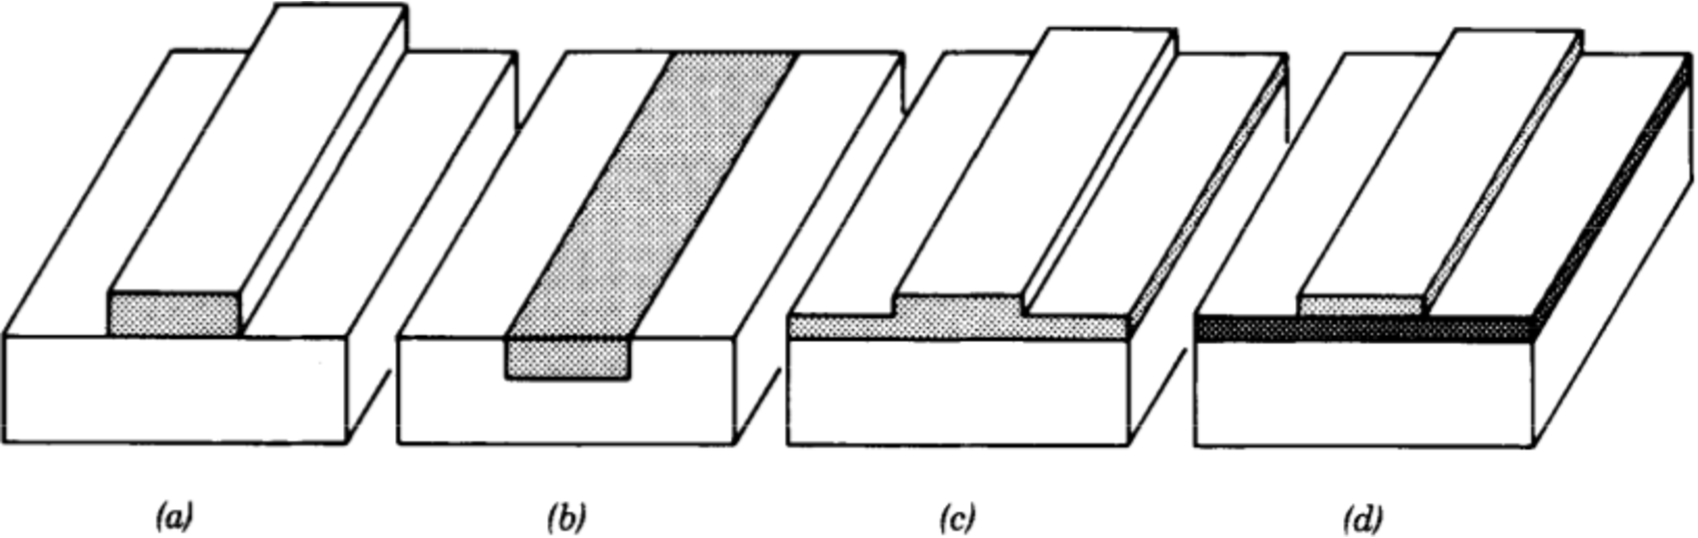
\includegraphics[scale=.4]{figures/WGtypes.pdf}
	\caption{Representation of a few types of 2D dielectric waveguides.
		Light is constrained in two direction and can only move forward or backward in the third direction.
		(a) strip, (b) embedded strip, (c) rib, (d) strip loaded \cite{Saleh1991}.
		}
	\label{fig:2DVG}
\end{figure}

Obviously, the versatility of straight (2D-) waveguides is limited.
Hence more complex structures such as bent waveguides have been developed.

\paragraph{Propagation of light inside waveguides\\}
\noindent Light propagates inside waveguides as superposition of transverse electro-magnetic (TEM) waves which keep reflecting on the interfaces of the core.
The result of the superposition is the so called \textit{mode}, which is expressed mathematically by
\begin{equation}
	\phi(\textbf{r}) = \phi_m\left( x, y \right) e^{i\left( \beta_m z - \omega t\right)}.
\end{equation}
$\phi_m\left( x, y \right)$ is the transverse field distribution, $z$ is the direction of propagation, $\beta_m$ is the propagation constant of the m-th mode, and $\omega=2\pi \nu$ is the angular frequency of light.
Each mode, identified by the $m$ idex, travels inside the waveguide with a certain propagation constant $\beta$ and maintaining a field distribution $\phi_m$.
Both of them depends on the materials and the geometry of the waveguide, however while $\beta_m$ decrease with increasing $m$ indexes, the features of the function $\phi_m$ grows in number.
Light either propagate in a manner described by a mode or superposition of modes or is rapidly scattered away.

The filed distribution of some of the first modes, in the simplest case of a slab waveguide, is represented in \autoref{fig:WGmodes} below.
\begin{figure}[ht]
	\centering
	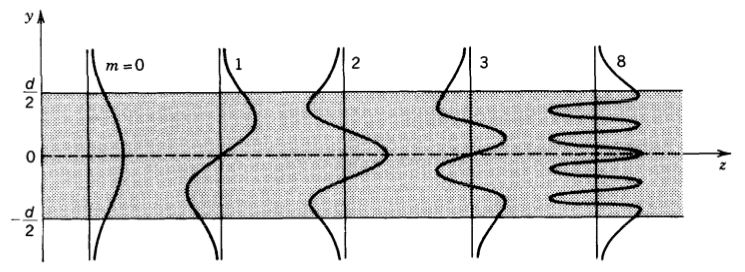
\includegraphics[scale=0.8]{figures/modes.png}
	\caption{Field distribution inside a slab waveguide.}
	\label{fig:WGmodes}
\end{figure}
The function inside the core is characterized by maxima, minima and nodes with a certain periodicity and the number of nodes (where the function is zero) is strictly linked to the index $m$.
Outside, the distribution of the field decays exponentially.
For waveguide with a 2D core, the field can be expected to be a multivariate version of the same or similar function.
However, differently from the analytical solution for slab waveguides, they are almost always found numerically.

The propagation constant can be written as
\begin{equation}
\beta_m = n_{eff} k_0
\end{equation}
where $k_0$ is the wavevector in vacuum and $n_{eff}$ is the \textit{effective refractive index} of the mode.
The value of this quantity is between the core refractive index and the cladding refractive index $n_L < n_{eff} < n_H$.
The physical interpretation of the effective index is that of an average refractive index \textit{felt} by the mode propagating as a whole, instead of a superposition of multiple TEM waves \textit{feeling} different refractive indexes depending on the specific medium in which they are propagating.
Similarly to the actual refractive index of materials, $n_{eff}$ is a complex number and the imaginary part is directly linked with the absorption properties of the materials.
Actually, a low imaginary part means that the material absorb less light and is therefore transparent.

All of these parameters which describe the propagation of light along the waveguide depends both on the materials and the geometry of the core and the cladding, but also on the frequency of light.
For dielectric waveguides, the fundamental mode ($m=0$) is always supported while higher modes might not be, depending both on the waveguides and on the frequency of light.
For this reason one distinguish \textit{single-mode} waveguides, which allow propagation for only the fundamental mode in a certain operative range of frequencies, from \textit{multi-mode} waveguides, which allow higher order modes to propagate.

\LARGE { mode propagation and GVD? } \normalsize

\subsection{Light coupling}
\label{ssec:light_coupling}
We covered how light travels inside a waveguide, now the problem on how to insert and extract light from it.
The process of inserting light into a waveguide is called \textit{coupling} and it often requires at the same time to extract light from another waveguide.

\subsubsection{End coupling}
\label{sssec:end_coupling}
The most naive way to insert light into a waveguide is obviously to use one of its ends.
This is achieved either by radiating a beam directly on the whole waveguide or by focusing it inside the core with some lensing mechanism (e.g. tapered optical fibers).

These methods are very simple, however they have a low coupling efficiency. % and are only able to access structures at perimeter of a chip.

\subsubsection{Grating coupling}
\label{sssec:grating_coupling}
% and prism coupling?
A more sophisticated way to couple light inside a waveguide is to use the so called \textit{grating coupler}.
A grating coupler is a periodic structure end coupled to a waveguide.
It is designed in a way such that light incident from free space above it, at a certain angle and with a specific wavelength, is coupled inside the waveguide.

\subsubsection{Evanescent coupling}
\label{sssec:evanescent_coupling}
Evanescent coupling exploits the fact that the field distribution outside the core decays exponentially to zero.
This means that when two waveguides are separated by a sufficiently small distance, the field distribution of one waveguide cannot decays sufficiently fast to zero and instead extends itself over the core of the second waveguide.
When this happens optical power can be transferred between the waveguides.
Therefore, if at the beginning light is propagating inside one waveguide, light is \textit{coupled} inside the other waveguide because its mode overlaps the core of the second waveguide.
Depending on the parameters of the problems, light can couple completely or partially between the waveguides.

This exchange of optical power is periodic with their length.

\subsection{Microring Optical Cavity}
\label{ssec:Microring_Optical_Cavity}
In integrated photonics the microring is an optical cavity made by bending a waveguide on itself.
To insert light into the cavity, the microring is often side coupled with one or two straight waveguides.
Light inserted from the different ports into the cavity interfere with itself, after a round trip, and with each other.
When the waves are in phase, they generate constructive interference and the energy stored in the cavity increases exponentially.
On the other hand, when the signals are out of phase, the interference is destructive and the energy stored in the cavity remains low.

In the simpler case, when there is only one waveguide side coupled to the resonator, the optical cavity has only two ports, which are usually called \textit{input} and \textit{through}.
This configuration is called \textit{All-Pass Filter}, because in the ideal case, where no losses happen, all the signal passes from the input to the through channels.
%All pass filter theory\\
All pass resonators have only one input and one output: light enters the resonator from the input and exits from the output, unless the device is used backwards or some specific phenomena happens (e.g. back scattering).

%1.2.3.2 Add-drop filter theory\\
\subsubsection{Add-drop filter theory}
\label{sssec:Add-drop_filter_theory}
By adding a secondary couple of input and output ports, one obtains the so called add-drop resonator.
The name comes from the fact that the secondary input is used as an add port to convey additional content to the output channel, while the drop port is used to take some of the light from the input channel.
Of course, light might also travel from the input to the output and from the add to the drop.
Whether light goes straight or passes through the resonator depends on the frequency of the signals and the relative position of the resonance.
Resonators with more than four ports are possible, however are very uncommon.

\begin{figure}[ht]
	\centering
	\tikzsetexternalprefix{tikz/}	% set subfolder
\tikzsetnextfilename{ADF}
\begin{tikzpicture}
	\newcommand\CENTRAL{193}
	\newcommand\START{193-5}
	\newcommand\STOP {193+7}
	\newcommand\CC{299792458}
	
	\begin{axis}[%
			axis x line*= bottom,
%			scaled x ticks = manual:{$+\SI{193}{\THz}$}{ \pgfmathparse{#1-\CENTRAL} },%
			xlabel = {Optical Frequency $\nu$ [$\si{\THz}$]},
			ylabel = {Transmission},
			legend columns=3,
			legend cell align=right,
			legend style={ at={(0.5,-0.22)}, anchor=north },
			width=\textwidth*0.75,%
			height=207pt,
			xmin= 188, xmax = 199,
			%
			% global plot definition
			domain = \START:\STOP,
			samples = 551,
			smooth,
			no markers,
			cycle multi list={
%					exotic\nextlist 
					color list\nextlist
					solid,densely dotted
					%[2 of]linestyles
				},
			]
				
		\foreach \TA/\LA/\Radius/\Neff in {0.85/0.9/5/3.826, 0.85/0.75/5/3.826 }{ %, 0.9/0.99/5/3.826
			\edef\temp{
				\noexpand\addlegendimage{empty legend}
				\noexpand\addlegendentry{$\tau=\TA,\gamma=\LA,R=\SI{\Radius}{\um}:$};
				\noexpand\addplot 
										{ + (1-\TA^2)^2 * \LA
											/ ( (1-\TA^2 * \LA)^2 	+ 4 * \TA^2 	* \LA *sin(deg(\Neff*pi*\Radius*2*pi*x*1e6/\CC))^2 )
										};
				\noexpand\addlegendentry{$D(\omega)$};
				\noexpand\addplot 
										{ + \TA^2 * ( (1- \LA)^2	+ 4 					* \LA *sin(deg(\Neff*pi*\Radius*2*pi*x*1e6/\CC))^2 )
											/ ( (1-\TA^2 * \LA)^2 	+ 4 * \TA^2 	* \LA *sin(deg(\Neff*pi*\Radius*2*pi*x*1e6/\CC))^2 )
										};
				\noexpand\addlegendentry{$T(\omega)$};
								}
			\temp
		}
		
		\draw [|<->|] (192.0446013229, 0.6) -- (194.5386870543, 0.6) node [midway, fill=white] {$FSR$};%0.5665693
	
		\draw [<-] (192.3, 0.283) -- (193.1,0.283) node [right] {$\Delta\omega$}; %0.5665693/2 = 0.283
		\draw [<-] (191.8, 0.283) -- (191,0.283) {};	
		
	\end{axis}
	
	\begin{axis}[
			width=\textwidth*0.75,%
			height=207pt,
			axis x line*= top,
			axis y line = none,
			xlabel = {Wavelength $\lambda$ [\si{\nm}]},
			xmin= 188, xmax = 199,
%			xmin= 150, xmax = 250,
%  		xtick = {187.37029,188.54872,189.74206,190.95061,192.17465,193.41449,194.67043,195.94278,197.23188,198.53805,199.86163},
			xtick = {187.37029,188.54872,189.74206,190.95061,192.17465,193.4143 ,194.67043,195.94278,197.2318 ,198.53805,199.86163},
%			xtick = {157.785504211, 171.309976, 187.37029, 199.86163, 214.13747, 230.609583077, 249.827048333},
%			scaled x ticks = manual:{$+\SI{1500}{\nm}$}{ \pgfkeys{/pgf/fpu}\pgfmathparse{(1e-3*\CC/#1) - 1500} },
			scaled x ticks = manual:{}{ \pgfkeys{/pgf/fpu}\pgfmathparse{(1e-3*\CC/#1)} },
		]
		\addplot[black, opacity=0, domain = \START:\STOP] {0}; %
	\end{axis}
\end{tikzpicture}
	\caption{Transmission spectra of microring resonators in Add-Drop Filter configuration for the through and drop ports.}
	\label{fig:ADF}
\end{figure}

\subsection{Nonlinear Perturbations}
\label{ssec:Nonlinear_Perturbations}

Comparison between nonlinear optics phenomena which affect a microring dynamic:
\begin{itemize}
\item TOC
\item FCD
\item FCA
\item Kerr
\item TPA
\end{itemize}

\section{Integrated photonics applied to ANNs}
\label{sec:Integrated_photonics_applied_to_ANNs}
Since our experiments are carried out in a time scale such that physics phenomena can be considered quasi-static, we obtain also that the only nonlinear effect non negligible is the thermo-optic effect.

\subsection{Weighted sum of inputs}
\label{ssec:Weighted_Sum_of_inputs}
This has already been demonstrated and integrated widely, so it will not be the focus of this work.
Two example are the banks of microring resonators and the MZ interferometers.

\subsection{Nonlinear Activation Function}
\label{ssec:Nonlinear_Activation_Function}
As opposed to the mechanism for weighted sum, an optical phenomenon for the activation function in an integrated photonic circuit has yet to be proposed.

\subsection{Simulations}
\label{ssec:Simulations}

\begin{figure}[ht]
	\centering
	\tikzsetexternalprefix{tikz/}	% set subfolder
\tikzsetnextfilename{bistability_test}
% This file was created by matplotlib2tikz v0.6.15.
\begin{tikzpicture}[baseline]
	
	\pgfplotstableread[col sep=tab, header=true]{tikz/foo.csv}\loadedtable
	
	\pgfplotstablegetcolsof{\loadedtable}
	\pgfmathparse{\pgfplotsretval - 1}
	\newcommand{\ncol}{\pgfmathresult}
	
	\definecolor{color1}{rgb}{1,0.498039215686275,0.0549019607843137}
	\definecolor{color6}{rgb}{0.890196078431372,0.466666666666667,0.76078431372549}
	\definecolor{color5}{rgb}{0.549019607843137,0.337254901960784,0.294117647058824}
	\definecolor{color2}{rgb}{0.172549019607843,0.627450980392157,0.172549019607843}
	\definecolor{color4}{rgb}{0.580392156862745,0.403921568627451,0.741176470588235}
	\definecolor{color3}{rgb}{0.83921568627451,0.152941176470588,0.156862745098039}
	\definecolor{color0}{rgb}{0.12156862745098,0.466666666666667,0.705882352941177}

\begin{axis}[
		title={Internal Power},
		xlabel={Pump Power $P$ $[mW]$},
		ylabel={Internal Power [a.u.*]},
		xmin=0.852408771935031, xmax=4.09941578936435,
		ymin=-3215.6821653405, ymax=90671.1511338174,
		tick align=outside,
		tick pos=left,
		width=\textwidth*0.75,%
		height=207pt,
		%x grid style={lightgray!92.02614379084967!black},
		%y grid style={lightgray!92.02614379084967!black},
		legend entries={
			{$\Delta\lambda$},
			{\SI{350}{\pm}},
			{\SI{379}{\pm}},
			{\SI{407}{\pm}},
			{\SI{436}{\pm}},
			{\SI{464}{\pm}},
			{\SI{493}{\pm}},
			{\SI{521}{\pm}},
			{\SI{550}{\pm}}
			},
		legend pos = outer north east,
		%legend cell align={left},
		%legend style={at={(1,-0.1)}, anchor=north west, draw=white!80.0!black},
		%legend columns=8
	]
	
	\addlegendimage{empty legend}
	\addlegendimage{mark=*, color0}
	\addlegendimage{mark=*, color1}
	\addlegendimage{mark=*, color2}
	\addlegendimage{mark=*, color3}
	\addlegendimage{mark=*, color4}
	\addlegendimage{mark=*, color5}
	\addlegendimage{mark=*, color6}
	\addlegendimage{mark=*, gray!99.6078431372549!black}

%\addlegendentry = {$\Delta\lambda$}
%\addlegendimage = {empty legend}
%\foreach \i in {1,2...,\pgfplotsretval-1} {
%	\addplot table [x index=0, y index=\i] {\loadedtable};
%	\pgfplotstablegetcolumnnamebyindex{\i}\of{\loadedtable}\to\colname
%	\addlegendentry = {\SI{\colname}{\pm}}
%	\addlegendimage = {mark=*, color\i}
%}

\addplot [semithick, color0, mark=*, mark size=1, mark options={solid}]
table {%
1 2182.13784798453
1.10996151344182 2732.06812562319
1.20997071148193 3301.35802903992
1.30232241935941 3891.75515464847
1.38854537026638 4505.26943967214
1.46971861477299 5144.22980210166
1.54663743906977 5811.35713826561
1.61990800024395 6509.85972553239
1.69000487886171 7243.55987029429
1.75730789900303 8017.0649998584
1.82212667320922 8836.00339261668
1.88471753176505 9707.35631717665
1.94529553946556 10639.9381155571
2.00404323735458 11645.110858216
2.06111713847338 12737.8851497554
2.11665264505793 13938.6847549387
2.1707678321628 15276.31091276
2.22356640163383 16793.2014266478
2.27514001850367 18555.3533357662
2.32557018064795 20672.1913566021
2.37492973084278 23336.6084050299
2.42328409142697 26875.9830526321
2.47069228134243 31476.9310455102
2.51720776067593 36046.2694806532
2.56287913716765 39544.1852080518
2.60775076129818 42181.9936544263
2.65186323070653 44282.0696014857
2.69525382027284 46032.9554507758
2.73795685083191 47541.7982041075
2.78000400689269 48873.3912118438
2.82142461172746 50069.4947595316
2.86224586662004 51158.5039921599
2.9024930598204 52160.5856929643
2.94218974976591 53090.5802810476
2.98135792633989 53959.7327474007
3.02001815330168 54776.7742586017
3.05818969450781 55548.625360946
3.09589062612293 56280.8689540435
3.13313793667592 56978.0778524274
3.16994761653247 57644.0474967912
3.20633473812108 58281.9649496754
3.24231352805431 58894.5341847922
3.27789743212414 59484.0704107321
3.31309917401337 60052.5723212442
3.34793080845022 60601.7782354623
3.38240376943561 61133.2101736674
3.41652891409018 61648.2089375426
3.45031656259774 62147.9622831466
3.48377653466154 62633.5277873525
3.51691818283855 63105.8515562808
3.54975042307237 63565.7836494865
3.58228176270719 64014.090916815
3.61452032623231 64451.4677214149
3.64647387897796 64878.5449862339
3.67814984895812 65295.8978439847
3.70955534703456 65704.052169585
3.74069718555709 66103.4901635271
3.77158189561844 66494.655157941
3.80221574304758 66877.9557805134
3.83260474325241 67253.7695572549
3.86275467501147 67622.4460626382
3.89267109330405 67984.3096727404
3.92235934125968 68339.6619855259
3.95182456129939 68688.7839488388
};
\addplot [semithick, color1, mark=*, mark size=1, mark options={solid}]
table {%
1 1940.07544411095
1.10996151344182 2423.22716305164
1.20997071148193 2920.70721201128
1.30232241935941 3433.61186262683
1.38854537026638 3963.17696183345
1.46971861477299 4510.8034528873
1.54663743906977 5078.08911859356
1.61990800024395 5666.86848769019
1.69000487886171 6279.26358787269
1.75730789900303 6917.74933289089
1.82212667320922 7585.2389829278
1.88471753176505 8285.19764576196
1.94529553946556 9021.7957820453
2.00404323735458 9800.12113436134
2.06111713847338 10626.4782986138
2.11665264505793 11508.8239192492
2.1707678321628 12457.4194811703
2.22356640163383 13485.848418119
2.27514001850367 14612.6752996465
2.32557018064795 15864.3096818447
2.37492973084278 17280.3143272715
2.42328409142697 18924.1988617378
2.47069228134243 20908.2895226999
2.51720776067593 23462.0392880969
2.56287913716765 27170.8381037511
2.60775076129818 33631.0297137638
2.65186323070653 40341.9479641702
2.69525382027284 44189.4013634534
2.73795685083191 46803.6856546889
2.78000400689269 48821.2416782276
2.82142461172746 50486.4792493101
2.86224586662004 51917.3882993097
2.9024930598204 53180.0763622241
2.94218974976591 54315.4654194578
2.98135792633989 55350.7465285369
3.02001815330168 56304.9665061537
3.05818969450781 57192.0231155222
3.09589062612293 58022.3918927019
3.13313793667592 58804.1805477364
3.16994761653247 59543.8034465492
3.20633473812108 60246.430206525
3.24231352805431 60916.2935960542
3.27789743212414 61556.9070656952
3.31309917401337 62171.2219851855
3.34793080845022 62761.7437447084
3.38240376943561 63330.6190515937
3.41652891409018 63879.7026494471
3.45031656259774 64410.6090421554
3.48377653466154 64924.7531439948
3.51691818283855 65423.3825577898
3.54975042307237 65907.6035338806
3.58228176270719 66378.4020054886
3.61452032623231 66836.6608209025
3.64647387897796 67283.1739473754
3.67814984895812 67718.6582859319
3.70955534703456 68143.7635642359
3.74069718555709 68559.0806667746
3.77158189561844 68965.1487014138
3.80221574304758 69362.4610174769
3.83260474325241 69751.4703637162
3.86275467501147 70132.5933346228
3.89267109330405 70506.2142143482
3.92235934125968 70872.6883067225
3.95182456129939 71232.3448615192
};
\addplot [semithick, color2, mark=*, mark size=1, mark options={solid}]
table {%
1 1732.97280209881
1.10996151344182 2160.25082035293
1.20997071148193 2598.25542831804
1.30232241935941 3047.68385058352
1.38854537026638 3509.3086372655
1.46971861477299 3983.98931489536
1.54663743906977 4472.68642687737
1.61990800024395 4976.47859191022
1.69000487886171 5496.5834020755
1.75730789900303 6034.38326074926
1.82212667320922 6591.45765894542
1.88471753176505 7169.62394084324
1.94529553946556 7770.98943472775
2.00404323735458 8398.01903253042
2.06111713847338 9053.62415924678
2.11665264505793 9741.28193834583
2.1707678321628 10465.1979664045
2.22356640163383 11230.5337188335
2.27514001850367 12043.7326151105
2.32557018064795 12913.002021987
2.37492973084278 13849.0520482085
2.42328409142697 14866.2785935804
2.47069228134243 15984.7629825415
2.51720776067593 17233.8916436386
2.56287913716765 18659.5263921909
2.60775076129818 20340.0938776341
2.65186323070653 22430.0792057072
2.69525382027284 25321.8960673326
2.73795685083191 30987.8016123129
2.78000400689269 44888.9927766667
2.82142461172746 48918.4586028915
2.86224586662004 51428.5184753255
2.9024930598204 53337.2501195886
2.94218974976591 54909.1358036994
2.98135792633989 56261.2528516411
3.02001815330168 57456.8190350748
3.05818969450781 58534.2614456403
3.09589062612293 59518.8696435552
3.13313793667592 60428.26786974
3.16994761653247 61275.282136951
3.20633473812108 62069.5689773745
3.24231352805431 62818.6003117727
3.27789743212414 63528.2893700834
3.31309917401337 64203.4049985116
3.34793080845022 64847.8553330121
3.38240376943561 65464.8876903212
3.41652891409018 66057.2328970549
3.45031656259774 66627.2118303121
3.48377653466154 67176.8154208414
3.51691818283855 67707.7658504522
3.54975042307237 68221.5639803765
3.58228176270719 68719.5266349635
3.61452032623231 69202.8162397473
3.64647387897796 69672.4646422314
3.67814984895812 70129.3924540031
3.70955534703456 70574.4248816071
3.74069718555709 71008.3048010219
3.77158189561844 71431.7036445875
3.80221574304758 71845.2304972518
3.83260474325241 72249.4397994264
3.86275467501147 72644.8378492904
3.89267109330405 73031.8883777777
3.92235934125968 73411.0173027476
3.95182456129939 73782.6168527726
};
\addplot [semithick, color3, mark=*, mark size=1, mark options={solid}]
table {%
1 1555.12712962575
1.10996151344182 1935.35022328765
1.20997071148193 2323.70064537386
1.30232241935941 2720.62917693881
1.38854537026638 3126.62808241723
1.46971861477299 3542.23655447464
1.54663743906977 3968.04710570885
1.61990800024395 4404.71310972971
1.69000487886171 4852.95775950785
1.75730789900303 5313.58477279263
1.82212667320922 5787.49128427383
1.88471753176505 6275.68348806087
1.94529553946556 6779.2957771205
2.00404323735458 7299.61438270963
2.06111713847338 7838.1068655017
2.11665264505793 8396.45931641251
2.1707678321628 8976.62387064854
2.22356640163383 9580.88022625359
2.27514001850367 10211.916530394
2.32557018064795 10872.9375886795
2.37492973084278 11567.812506292
2.42328409142697 12301.2807338782
2.47069228134243 13079.2472517646
2.51720776067593 13909.2186734183
2.56287913716765 14800.9715720034
2.60775076129818 15767.623259535
2.65186323070653 16827.4446215626
2.69525382027284 18007.1530903572
2.73795685083191 19348.4800019746
2.78000400689269 20923.1011850703
2.82142461172746 22874.1137116357
2.86224586662004 25581.679254139
2.9024930598204 32373.8833560084
2.94218974976591 53685.3764633791
2.98135792633989 56034.1288896655
3.02001815330168 57820.9838468359
3.05818969450781 59297.9114358345
3.09589062612293 60573.1864351054
3.13313793667592 61704.6888586915
3.16994761653247 62727.4816976698
3.20633473812108 63664.6266831185
3.24231352805431 64532.2068880532
3.27789743212414 65341.9425439077
3.31309917401337 66102.6722811745
3.34793080845022 66821.2474128613
3.38240376943561 67503.0999560958
3.41652891409018 68152.6186366019
3.45031656259774 68773.406464817
3.48377653466154 69368.4623655541
3.51691818283855 69940.3124659625
3.54975042307237 70491.1070517066
3.58228176270719 71022.6935267439
3.61452032623231 71536.6722322788
3.64647387897796 72034.4397820577
3.67814984895812 72517.2231554371
3.70955534703456 72986.1068373264
3.74069718555709 73442.0546571947
3.77158189561844 73885.9275378199
3.80221574304758 74318.4980334294
3.83260474325241 74740.4623689852
3.86275467501147 75152.4504450848
3.89267109330405 75555.034238381
3.92235934125968 75948.7348944082
3.95182456129939 76334.028743014
};
\addplot [semithick, color4, mark=*, mark size=1, mark options={solid}]
table {%
1 1401.7392420467
1.10996151344182 1742.05447923165
1.20997071148193 2088.60129970629
1.30232241935941 2441.67621144985
1.38854537026638 2801.59908560004
1.46971861477299 3168.71577477143
1.54663743906977 3543.40111578359
1.61990800024395 3926.06239167527
1.69000487886171 4317.14333702743
1.75730789900303 4717.12879862109
1.82212667320922 5126.55018167644
1.88471753176505 5545.99185421269
1.94529553946556 5976.0987168996
2.00404323735458 6417.58521344896
2.06111713847338 6871.24612225125
2.11665264505793 7337.96958510755
2.1707678321628 7818.75295467511
2.22356640163383 8314.72224806523
2.27514001850367 8827.15625233288
2.32557018064795 9357.51670762848
2.37492973084278 9907.48654853509
2.42328409142697 10479.0189765846
2.47069228134243 11074.4013469418
2.51720776067593 11696.3396961176
2.56287913716765 12348.0726453624
2.60775076129818 13033.5281305727
2.65186323070653 13757.5443237197
2.69525382027284 14526.1899146087
2.73795685083191 15347.2441508942
2.78000400689269 16230.9456576159
2.82142461172746 17191.2192207557
2.86224586662004 18247.8134492887
2.9024930598204 19430.3365989971
2.94218974976591 20786.7549552248
2.98135792633989 22404.3765552702
3.02001815330168 24477.132776658
3.05818969450781 27686.4341351164
3.09589062612293 60604.7367382226
3.13313793667592 62267.3306556756
3.16994761653247 63651.8767800161
3.20633473812108 64854.0003360527
3.24231352805431 65925.1989624745
3.27789743212414 66896.8638024415
3.31309917401337 67789.7512506825
3.34793080845022 68618.4032399159
3.38240376943561 69393.4596711254
3.41652891409018 70122.9731701597
3.45031656259774 70813.2057695201
3.48377653466154 71469.1366375532
3.51691818283855 72094.7992028596
3.54975042307237 72693.5127477348
3.58228176270719 73268.04615849
3.61452032623231 73820.7365353523
3.64647387897796 74353.577049637
3.67814984895812 74868.2831356681
3.70955534703456 75366.343267635
3.74069718555709 75849.0584399384
3.77158189561844 76317.5732904656
3.80221574304758 76772.9009091922
3.83260474325241 77215.9428404241
3.86275467501147 77647.5053551995
3.89267109330405 78068.3128118444
3.92235934125968 78479.018719511
3.95182456129939 78880.2149507901
};
\addplot [semithick, color5, mark=*, mark size=1, mark options={solid}]
table {%
1 1268.82868775917
1.10996151344182 1575.05802024631
1.20997071148193 1886.12026197023
1.30232241935941 2202.21379773944
1.38854537026638 2523.5504741739
1.46971861477299 2850.35689401489
1.54663743906977 3182.87587513696
1.61990800024395 3521.36809814379
1.69000487886171 3866.11397301945
1.75730789900303 4217.4157647887
1.82212667320922 4575.60001730141
1.88471753176505 4941.02033443108
1.94529553946556 5314.06057831588
2.00404323735458 5695.1385694657
2.06111713847338 6084.71038352431
2.11665264505793 6483.27536643047
2.1707678321628 6891.38202520844
2.22356640163383 7309.63497755628
2.27514001850367 7738.70321414165
2.32557018064795 8179.32997495534
2.37492973084278 8632.34465296927
2.42328409142697 9098.67724862147
2.47069228134243 9579.37607223338
2.51720776067593 10075.6296358352
2.56287913716765 10588.794003145
2.60775076129818 11120.4273476226
2.65186323070653 11672.3341837221
2.69525382027284 12246.6227764755
2.73795685083191 12845.7808515076
2.78000400689269 13472.7772471925
2.82142461172746 14131.2012233633
2.86224586662004 14825.4579311768
2.9024930598204 15561.0503423298
2.94218974976591 16344.9992760867
2.98135792633989 17186.4940437196
3.02001815330168 18097.9494922264
3.05818969450781 19096.8290326469
3.09589062612293 20209.0416065191
3.13313793667592 21475.970206772
3.16994761653247 22971.3891448233
3.20633473812108 24853.4294810608
3.24231352805431 27628.5741492578
3.27789743212414 67971.5517060323
3.31309917401337 69105.1416733301
3.34793080845022 70120.0946247003
3.38240376943561 71044.1745834219
3.41652891409018 71895.906585186
3.45031656259774 72688.3618266287
3.48377653466154 73431.1596717701
3.51691818283855 74131.6157929157
3.54975042307237 74795.4428143908
3.58228176270719 75427.1994959916
3.61452032623231 76030.5904912877
3.64647387897796 76608.6731994837
3.67814984895812 77164.0045519713
3.70955534703456 77698.7477761974
3.74069718555709 78214.7516479251
3.77158189561844 78713.6104264719
3.80221574304758 79196.7099098472
3.83260474325241 79665.2633847461
3.86275467501147 80120.339956786
3.89267109330405 80562.8872403561
3.92235934125968 80993.7496498591
3.95182456129939 81413.6833305709
};
\addplot [semithick, color6, mark=*, mark size=1, mark options={solid}]
table {%
1 1153.11534113191
1.10996151344182 1430.03226695262
1.20997071148193 1710.73804990963
1.30232241935941 1995.36761972763
1.38854537026638 2284.06383596786
1.46971861477299 2576.97814784539
1.54663743906977 2874.271324898
1.61990800024395 3176.11426828301
1.69000487886171 3482.68891680214
1.75730789900303 3794.18925621961
1.82212667320922 4110.82245204988
1.88471753176505 4432.81012075285
1.94529553946556 4760.38976134927
2.00404323735458 5093.81637550133
2.06111713847338 5433.36430322558
2.11665264505793 5779.32931126422
2.1707678321628 6132.03098200405
2.22356640163383 6491.81544913815
2.27514001850367 6859.0585527477
2.32557018064795 7234.16948577099
2.37492973084278 7617.59503665301
2.42328409142697 8009.82454518515
2.47069228134243 8411.39572435789
2.51720776067593 8822.9015440492
2.56287913716765 9244.9984176772
2.60775076129818 9678.41600447315
2.65186323070653 10123.9690407346
2.69525382027284 10582.5717252035
2.73795685083191 11055.255374458
2.78000400689269 11543.1902961492
2.82142461172746 12047.7131731641
2.86224586662004 12570.3617592033
2.9024930598204 13112.9194050828
2.94218974976591 13677.4730410114
2.98135792633989 14266.4899249147
3.02001815330168 14882.92113088
3.05818969450781 15530.3440849035
3.09589062612293 16213.1637448906
3.13313793667592 16936.9048102428
3.16994761653247 17708.6507936515
3.20633473812108 18537.731333299
3.24231352805431 19436.8536726255
3.27789743212414 20424.0877878307
3.31309917401337 21526.6517346132
3.34793080845022 22789.0048056135
3.38240376943561 24293.3410848102
3.41652891409018 26228.6066943418
3.45031656259774 29348.8257048927
3.48377653466154 75171.1397221552
3.51691818283855 75984.6568808932
3.54975042307237 76743.4666071406
3.58228176270719 77456.2449920176
3.61452032623231 78129.6279619962
3.64647387897796 78768.8222956222
3.67814984895812 79377.9997469359
3.70955534703456 79960.5631547749
3.74069718555709 80519.3292809379
3.77158189561844 81056.6605048151
3.80221574304758 81574.5604661358
3.83260474325241 82074.7454388648
3.86275467501147 82558.6984882122
3.89267109330405 83027.7111994293
3.92235934125968 83482.9163354476
3.95182456129939 83925.3136700693
};
\addplot [semithick, gray!99.6078431372549!black, mark=*, mark size=1, mark options={solid}]
table {%
1 1051.90116643941
1.10996151344182 1303.44726288011
1.20997071148193 1557.99394172329
1.30232241935941 1815.63441347309
1.38854537026638 2076.46666063304
1.46971861477299 2340.59378187961
1.54663743906977 2608.12436994593
1.61990800024395 2879.17292492343
1.69000487886171 3153.86030778706
1.75730789900303 3432.31424093356
1.82212667320922 3714.66985891778
1.88471753176505 4001.07031664975
1.94529553946556 4291.66746463481
2.00404323735458 4586.622597123
2.06111713847338 4886.1072842512
2.11665264505793 5190.30430224765
2.1707678321628 5499.40867237775
2.22356640163383 5813.62882592496
2.27514001850367 6133.18791706005
2.32557018064795 6458.32530267821
2.37492973084278 6789.29821739155
2.42328409142697 7126.38367974316
2.47069228134243 7469.88066200891
2.51720776067593 7820.1125779211
2.56287913716765 8177.43014050562
2.60775076129818 8542.21466092436
2.65186323070653 8914.88187908926
2.69525382027284 9295.88642441276
2.73795685083191 9685.72704972988
2.78000400689269 10084.9527957754
2.82142461172746 10494.1703087648
2.86224586662004 10914.0525718883
2.9024930598204 11345.3494129332
2.94218974976591 11788.9002336084
2.98135792633989 12245.6495758424
3.02001815330168 12716.6663249425
3.05818969450781 13203.1676488722
3.09589062612293 13706.549171899
3.13313793667592 14228.4234937297
3.16994761653247 14770.6700428606
3.20633473812108 15335.5006187596
3.24231352805431 15925.5470950771
3.27789743212414 16543.9811598262
3.31309917401337 17194.6816380418
3.34793080845022 17882.4746784895
3.38240376943561 18613.4896944253
3.41652891409018 19395.7073085347
3.45031656259774 20239.8430326763
3.48377653466154 21160.8577524495
3.51691818283855 22180.7408622233
3.54975042307237 23334.1838011124
3.58228176270719 24681.9491843409
3.61452032623231 26350.5329837158
3.64647387897796 28717.9644245379
3.67814984895812 81469.8024553932
3.70955534703456 82117.9322483101
3.74069718555709 82734.115466073
3.77158189561844 83322.1707454383
3.80221574304758 83885.2242523683
3.83260474325241 84425.872718139
3.86275467501147 84946.3003285067
3.89267109330405 85448.3644825201
3.92235934125968 85933.6599597318
3.95182456129939 86403.5678020375
};
\end{axis}

\end{tikzpicture}
	\caption{}
%	\label{fig:bist_test}
\end{figure}

\begin{figure}[ht]
	\centering
	\tikzsetexternalprefix{tikz/}	% set subfolder
\tikzsetnextfilename{bistability_test2}
% This file was created by matplotlib2tikz v0.6.15.

\newcommand{\downfile}[1]{
    \pgfplotstableread[col sep=tab, header=true]{#1}{\table}
    \pgfplotstablegetcolsof{#1}
    \pgfmathtruncatemacro\numberofcols{\pgfplotsretval - 1}
    \pgfplotsinvokeforeach{1,...,\numberofcols}{
        \pgfplotstablegetcolumnnamebyindex{##1}\of{\table}\to{\colname}
        \addplot [name path=down##1, semithick, color##1, mark=*, mark size=1, mark options={solid}]%
        		table [x index= 0, y index=##1] {#1};
        \addlegendentryexpanded{ \colname }
    }
}

\newcommand{\upfile}[1]{
    \pgfplotstableread[col sep=tab, header=true]{#1}{\table}
    \pgfplotstablegetcolsof{#1}
    \pgfmathtruncatemacro\numberofcols{\pgfplotsretval - 1}
    \pgfplotsinvokeforeach{1,...,\numberofcols}{
        \pgfplotstablegetcolumnnamebyindex{##1}\of{\table}\to{\colname}
        \addplot [name path=up##1, semithick, color##1, mark=*, mark size=1, mark options={solid}]%
        		table [x index= 0, y index=##1] {#1};
    }
}

\begin{tikzpicture}[baseline]

	\definecolor{color1}{rgb}{0.12156862745098,0.466666666666667,0.705882352941177}
	\definecolor{color2}{rgb}{1,0.498039215686275,0.0549019607843137}
	\definecolor{color3}{rgb}{0.172549019607843,0.627450980392157,0.172549019607843}
	\definecolor{color4}{rgb}{0.83921568627451,0.152941176470588,0.156862745098039}
	\definecolor{color5}{rgb}{0.580392156862745,0.403921568627451,0.741176470588235}
	\definecolor{color6}{rgb}{0.549019607843137,0.337254901960784,0.294117647058824}
	\definecolor{color7}{rgb}{0.890196078431372,0.466666666666667,0.76078431372549}
	\definecolor{color8}{rgb}{0.45,0.45,0.45}
	\definecolor{color9}{rgb}{0.25,0.25,0.99}
	
	\begin{axis}[
			title={Transmitted Power to Drop Channel},
			xlabel={Pump Power [\si{mW}]},
			ylabel={$D(\lambda)$ [\si{\mW}]},
%			tick align=outside,
%			tick pos=left,
			width=\textwidth*0.75,%
			height=207pt,
			legend pos = outer north east,
			%cycle list name=color list,
			forget plot style={opacity=0.4},
		]
		\addlegendentry{\hspace{-.6cm}$\Delta\lambda$ in \si{\pm}}
		\addlegendimage{empty legend};
		
		\upfile{tikz/upwards.csv}
		\downfile{tikz/downwards.csv}

    \addplot [fill=color1, opacity=0.2] fill between [of=up1 and down1];
    \addplot [fill=color2, opacity=0.2] fill between [of=up2 and down2];
    \addplot [fill=color3, opacity=0.2] fill between [of=up3 and down3];
    \addplot [fill=color4, opacity=0.2] fill between [of=up4 and down4];
    \addplot [fill=color5, opacity=0.2] fill between [of=up5 and down5];
    \addplot [fill=color6, opacity=0.2] fill between [of=up6 and down6];
    \addplot [fill=color7, opacity=0.2] fill between [of=up7 and down7];
    \addplot [fill=color8, opacity=0.2] fill between [of=up8 and down8];
    \addplot [fill=color9, opacity=0.2] fill between [of=up9 and down9];
	\end{axis}
\end{tikzpicture}
	\caption{}
%	\label{fig:bist_test}
\end{figure}